\documentclass[12pt]{article}
\usepackage{sbc-template}

\usepackage[utf8]{inputenc}
\usepackage[T1]{fontenc}
\usepackage{cite}
\usepackage{amsmath,amssymb,amsfonts}
\usepackage{graphicx}
\usepackage{tabularray} % pretty tables
\usepackage{textcomp}
\usepackage{xcolor}
\usepackage{comment}
\usepackage{mathtools}
\usepackage{xspace}
\usepackage{multirow}
\usepackage{float} % opção H para figuras/tabelas
\usepackage{boldline}
\usepackage{scalefnt}
\usepackage{colortbl}
\usepackage{booktabs} % tabelas
\usepackage[tight,footnotesize]{subfigure}
\usepackage{hyperref} % urls nas referências
\usepackage{relsize}
\usepackage{makecell}
\usepackage{arydshln} % linhas tracejadas em tabelas

\usepackage{array}
\usepackage{calrsfs}
\DeclareMathAlphabet{\pazocal}{OMS}{zplm}{m}{n}

% centered fixed-width column used by some tables
\newcolumntype{C}[1]{>{\centering\arraybackslash}m{#1}}

% Rótulos em português (o template não carrega babel)
\renewcommand{\figurename}{Figura}
\renewcommand{\tablename}{Tabela}
\renewcommand{\refname}{Referências}


\sloppy

\title{Aprendizado Federado com Privacidade Diferencial para Manutenção Preditiva}

\author{Vinicius Trindade Dias Abel\inst{1}, Victor Gabriel Moura Oliveira\inst{1}, Julio Assis Souza Amorim\inst{1}}

\address{Depto. de Ciência da Computação (DCC) -- UFMG
\email{\{viniciustda, victorgabrielengsis, gmndaxdo@ufmg.br\}}
}

\begin{document}

\maketitle
\pagestyle{myheadings}

\begin{abstract}
Predictive maintenance relies on sensor data that is distributed across factories
and carries sensitive information, which discourages centralizing it on a single
server. We apply federated learning to train a failure classifier without moving
the factory data, and we add differential privacy through the Gaussian mechanism
with L2 sensitivity clipping, so that the shared parameters do not reveal individual
records. We measure the privacy--utility trade-off by varying the privacy budget
$\epsilon$, and we quantify the protection with a calibrated membership inference
attack (LiRA). The federated model reaches $0.818$ accuracy without protection and
$0.537$ at $\epsilon=0.5$, while differential privacy lowers the attack AUC from
$0.528$ to around $0.508$, close to the random baseline of $0.500$.
\end{abstract}

\begin{resumo}
A manutenção preditiva depende de dados de sensores que ficam distribuídos entre
fábricas e carregam informação sensível, o que restringe a reunião desses dados num
servidor único. Este trabalho aplica aprendizado federado para treinar um
classificador de falhas sem mover os dados das fábricas e acrescenta privacidade
diferencial, por meio do mecanismo gaussiano com recorte da norma L2, para impedir
que os parâmetros compartilhados revelem registros individuais. A avaliação mede o
compromisso entre privacidade e utilidade ao variar o orçamento $\epsilon$ e
quantifica a proteção com um ataque de inferência de pertencimento calibrado (LiRA).
O modelo federado atinge $0{,}818$ de acurácia sem proteção e $0{,}537$ em
$\epsilon=0{,}5$, enquanto a privacidade diferencial reduz a AUC do ataque de
$0{,}528$ para cerca de $0{,}508$, próxima do acaso ($0{,}500$).
\end{resumo}

\section{Introdução} \label{sec:intro}

A manutenção preditiva antecipa falhas de equipamentos industriais a partir de
leituras de sensores, o que reduz paradas não planejadas e custos de operação.
Sensores de temperatura, torque, rotação e desgaste descrevem o estado de cada
máquina, e um classificador aprende a relação entre esses sinais e a ocorrência de
falha. A qualidade dessa previsão depende do volume e da diversidade dos dados de
treino, que costumam pertencer a fábricas diferentes.

Esses dados, porém, carregam informação sensível e ficam distribuídos entre as
fábricas, o que restringe a reunião deles num servidor central. Registros de
operação revelam padrões de produção e segredos industriais, e legislações de
proteção de dados, como a LGPD, limitam o compartilhamento. A centralização, além do
risco jurídico, exige a transferência e o armazenamento de grandes volumes de dados,
custo que nem sempre compensa.

O aprendizado federado responde a essa restrição. Cada fábrica treina um modelo
local e envia ao servidor os parâmetros, nunca os dados brutos
\cite{mcmahan2017fedavg}. O servidor agrega os parâmetros num modelo global e o
devolve às fábricas, ao longo de várias rodadas. A troca de parâmetros, no entanto, ainda
revela informação: estudos demonstram que um adversário infere registros do treino a
partir do modelo \cite{shokri2017membership}. O aprendizado federado, sozinho, não
oferece garantia formal de privacidade.

A privacidade diferencial resolve essa limitação ao acrescentar ruído calibrado aos
parâmetros antes do envio, o que torna improvável a distinção de qualquer registro
individual \cite{dwork2014foundations}. Este trabalho constrói um sistema de
aprendizado federado com privacidade diferencial para a previsão de falhas no
conjunto AI4I 2020 \cite{matzka2020explainable} e mede o efeito da proteção sobre a
utilidade do modelo. O mecanismo gaussiano, com recorte da norma L2 e ruído
proporcional ao orçamento $\epsilon$, protege a participação de cada fábrica a cada
rodada. Um ataque de inferência de pertencimento calibrado \cite{carlini2022membership}
quantifica a proteção e confirma o seu efeito. Este trabalho apresenta quatro
resultados: o mecanismo de privacidade diferencial sobre o classificador federado; a
medição do compromisso entre privacidade e utilidade ao variar $\epsilon$; a
avaliação da proteção por meio do ataque LiRA; e um ambiente reproduzível em
contêineres Docker que executa todo o experimento.

A Seção \ref{sec:trabRel} relaciona o trabalho com a literatura. A Seção \ref{sec:model}
descreve a arquitetura federada e o mecanismo de privacidade diferencial. A Seção
\ref{sec:aval} detalha o conjunto de dados, o protocolo de avaliação e o ataque. A
Seção \ref{sec:results} reúne os resultados, e a Seção \ref{sec:conc} resume as
conclusões.

\section{Trabalhos relacionados} \label{sec:trabRel}

O aprendizado federado treina um modelo compartilhado sobre dados que ficam nos
clientes. O algoritmo FedAvg calcula a média ponderada dos parâmetros locais a cada
rodada e reduz a frequência de comunicação com o servidor \cite{mcmahan2017fedavg}.
O arcabouço Flower implementa esse protocolo e organiza a troca de mensagens entre o
servidor e os clientes \cite{beutel2020flower}, e é a base da arquitetura deste
trabalho.

A privacidade diferencial formaliza o limite de informação que um resultado revela
sobre um registro individual \cite{dwork2014foundations}. O mecanismo gaussiano
alcança esse limite ao somar ruído proporcional à sensibilidade da função. No
aprendizado profundo, o algoritmo DP-SGD recorta o gradiente de cada exemplo e soma
ruído a cada passo \cite{abadi2016deep}, e a mesma ideia protege modelos de
linguagem treinados de forma federada \cite{mcmahan2018learning}. Este trabalho
aplica esse mecanismo aos parâmetros do classificador antes da agregação.

O ataque de inferência de pertencimento decide se um registro específico participou
do treino, e serve como teste empírico de privacidade \cite{shokri2017membership}. A
versão LiRA calibra essa decisão com modelos de referência que estimam a
distribuição de perda de um exemplo quando ele não pertence ao treino, o que aumenta a
precisão do ataque \cite{carlini2022membership}. A avaliação deste trabalho adota o
LiRA para medir a proteção do mecanismo.

O conjunto AI4I 2020 reproduz dados de manutenção preditiva de equipamentos
industriais e rotula cada registro como falha ou operação normal
\cite{matzka2020explainable}. A biblioteca scikit-learn fornece o classificador e as
métricas de avaliação \cite{pedregosa2011scikit}.

\section{Modelo} \label{sec:model}

\subsection{Arquitetura federada}

A arquitetura reúne três clientes e um servidor central. Cada cliente representa uma
fábrica e tem uma fatia disjunta do conjunto de dados, o que reproduz a separação
física dos registros. O servidor coordena 20 rodadas de treino. A cada rodada, cada
cliente ajusta um modelo de regressão logística sobre os próprios dados e envia os
parâmetros ao servidor. O servidor agrega os parâmetros pela média ponderada no
número de amostras (FedAvg) e devolve o modelo global para a rodada seguinte. O
arcabouço Flower gerencia a comunicação por gRPC, e contêineres Docker isolam cada
fábrica e o servidor.

A regressão logística atende a esse cenário por dois motivos: o vetor de parâmetros
tem dimensão baixa, o que facilita o recorte da norma e o controle do ruído; e o
treino aceita o ajuste incremental entre rodadas. O peso de classe equilibra a
influência das falhas, raras no conjunto, sobre a função de perda.

\subsection{Privacidade diferencial}

Um mecanismo aleatório $\mathcal{M}$ satisfaz $(\epsilon,\delta)$-privacidade
diferencial quando, para quaisquer dois conjuntos vizinhos $D$ e $D'$ que diferem em
um registro e para qualquer subconjunto $S$ de saídas,
\begin{equation}
\Pr[\mathcal{M}(D)\in S] \le e^{\epsilon}\,\Pr[\mathcal{M}(D')\in S] + \delta .
\label{eq:dp}
\end{equation}
O parâmetro $\epsilon$ limita o ganho de informação sobre um registro, e $\delta$
permite uma folga de probabilidade. Um $\epsilon$ menor aproxima as duas
distribuições e aumenta a privacidade.

Cada cliente aplica o mecanismo aos parâmetros do modelo (não aos atributos nem aos dados brutos), após o treino local e antes do envio ao servidor. O mecanismo gaussiano protege os parâmetros em duas etapas. A primeira recorta o
vetor de parâmetros $v=[\,\mathrm{coef},\,\mathrm{intercepto}\,]$ para que a norma L2
não ultrapasse um limite $C$, o que define a sensibilidade do envio. A segunda soma ruído
gaussiano de desvio-padrão $\sigma$ a cada componente, com
\begin{equation}
\sigma = \frac{C}{\epsilon}\,\sqrt{\ln(1/\delta)} .
\label{eq:sigma}
\end{equation}
A Equação \ref{eq:sigma} liga o ruído ao orçamento: um $\epsilon$ menor aumenta
$\sigma$ e reforça a proteção, ao custo de maior distorção dos parâmetros.

A Equação \ref{eq:sigma} adota uma calibração simplificada do mecanismo gaussiano, com
garantia formal no regime $\epsilon \le 1$. Vale destacar dois pontos. O recorte do
vetor à bola de raio $C$ limita a sensibilidade L2 ao diâmetro $2C$ no pior caso, e a
calibração usa $C$ como aproximação. A forma clássica de Dwork e Roth
\cite{dwork2014foundations} pede $\sigma \ge (C/\epsilon)\sqrt{2\ln(1{,}25/\delta)}$, um
pouco acima da Equação \ref{eq:sigma}, de modo que o $\epsilon$ efetivo fica acima do
nominal. Para $\epsilon > 1$, avaliado aqui para explorar o compromisso entre privacidade e
utilidade, uma garantia estrita exigiria o mecanismo gaussiano analítico
\cite{balle2018analytic} ou a contabilidade por privacidade diferencial de Rényi
\cite{mironov2017renyi}.

O orçamento $\epsilon$ vale para uma rodada. Ao longo de $k$ rodadas, a composição
sequencial soma o gasto e limita a privacidade total a $k\cdot\epsilon$ no pior caso.
O protocolo de 20 rodadas com $\epsilon=1$ por rodada, portanto, consome um orçamento
total de 20. A Seção \ref{sec:results} apresenta esse total para cada configuração.

A Figura \ref{alg:dp} resume o procedimento que cada cliente executa antes do envio.
O recorte fixa a sensibilidade, e o ruído gaussiano da Equação \ref{eq:sigma}
garante a proteção formal sobre o vetor recortado.

\begin{figure}[H]
\centering
\fbox{%
\begin{minipage}{0.90\linewidth}
\small
\textbf{Procedimento} \textsc{AplicarDP}$(\mathrm{coef},\ \mathrm{intercepto},\ C,\ \epsilon,\ \delta)$\\[3pt]
\textbf{Entrada:} parâmetros locais; limite de norma $C$; orçamento $\epsilon$; folga $\delta$.\\
\textbf{Saída:} parâmetros com privacidade diferencial.\\[4pt]
1.\quad $v \leftarrow$ concatena$(\mathrm{coef},\ \mathrm{intercepto})$ \hfill {\itshape // vetor único}\\
2.\quad $n \leftarrow \lVert v \rVert_2$\\
3.\quad \textbf{se} $n > C$ \textbf{então} $v \leftarrow v \cdot (C / n)$ \hfill {\itshape // recorte da sensibilidade}\\
4.\quad $\sigma \leftarrow (C/\epsilon)\,\sqrt{\ln(1/\delta)}$\\
5.\quad $v \leftarrow v + \mathcal{N}(0,\ \sigma^2 I)$ \hfill {\itshape // ruído gaussiano}\\
6.\quad \textbf{devolve} restaura$(v)$
\end{minipage}}
\caption{Mecanismo gaussiano que cada cliente aplica aos parâmetros antes do envio ao servidor.}
\label{alg:dp}
\end{figure}

\section{Avaliação} \label{sec:aval}

\subsection{Conjunto de dados}

O conjunto AI4I 2020 reúne 10000 registros de operação de máquinas industriais \cite{matzka2020explainable}. Cada registro traz seis atributos de entrada (o tipo de produto e as leituras de temperatura do ar, temperatura do processo, rotação, torque e desgaste da ferramenta) e um rótulo binário que indica falha ou operação normal. As falhas respondem por cerca de $3{,}4\%$ das amostras, o que caracteriza um conjunto desbalanceado.

O pré-processamento prepara os atributos para o classificador. O atributo categórico de tipo (L, M, H) recebe a codificação 0, 1 e 2. A seleção mantém os seis atributos de sensores e o rótulo agregado de falha, e descarta o identificador, o código do produto e os cinco modos de falha individuais. Uma padronização $z$-score coloca os atributos na mesma escala, necessária porque os sensores têm faixas diferentes. O peso de classe balanceado, na função de perda, trata a raridade das falhas.

A simulação reproduz a separação física dos dados entre as fábricas. Um embaralhamento com semente fixa (42) vem antes da divisão dos 10000 registros em três fatias disjuntas e de tamanho próximo (3334, 3333 e 3333). A divisão aleatória mantém a mesma distribuição em cada fatia: cada fábrica recebe perto de $3{,}4\%$ de falhas. O conjunto fica, assim, balanceado entre as fábricas (mesma proporção de classes) e desbalanceado dentro de cada uma, com a falha rara em todas.

\subsection{Modelo e protocolo}

Cada fábrica treina uma regressão logística com peso de classe balanceado e ajuste
incremental, e o servidor combina os modelos por FedAvg ao longo de 20 rodadas. O
sistema implantado executa esse protocolo sobre o arcabouço Flower em contêineres Docker,
descrito na Seção \ref{sec:model}. Os resultados a seguir vêm de um arcabouço de avaliação
que reproduz o mesmo protocolo num único processo e reaproveita o mesmo código de
privacidade diferencial (o módulo \texttt{dp\_utils}), o que mantém o mecanismo idêntico ao
do sistema implantado, com a agregação FedAvg reimplementada para concentrar todo o
experimento. Esse arcabouço varia uma variável de
cada vez, entre o orçamento $\epsilon$, o limite de norma $C$, a folga $\delta$ e o número
de rodadas, com as outras fixas no padrão ($C=1$, $\epsilon=1$, $\delta=10^{-5}$,
20 rodadas). Como o ruído é aleatório, cada configuração com privacidade diferencial
repete oito execuções, e a média estabiliza a métrica.

O intervalo de $\epsilon$ avaliado para a utilidade, de $0{,}5$ a 8, vem da relação entre ruído e orçamento. O desvio-padrão $\sigma$ cresce com $1/\epsilon$ (Equação \ref{eq:sigma}): com $C=1$, a norma dos parâmetros fica limitada a um, enquanto $\epsilon=0{,}5$ já injeta $\sigma \approx 6{,}8$ e $\epsilon=0{,}01$ levaria $\sigma$ a cerca de 339. Abaixo de $\epsilon \approx 0{,}5$, portanto, o ruído supera o sinal e a acurácia cai para o acaso, sem informação a observar. O intervalo de $0{,}5$ a 8 cobre a transição da utilidade, do quase-acaso à recuperação parcial. A avaliação do ataque segue a direção oposta e estende $\epsilon$ até 64, com $\sigma \approx 0{,}05$, para testar a privacidade mesmo quase sem ruído.

\subsection{Métricas de utilidade}

A avaliação apresenta três métricas. A acurácia global mede o acerto sobre todas as
amostras, mas engana num conjunto desbalanceado, pois um classificador que prevê
sempre ``normal'' alcança valor alto sem detectar nenhuma falha. O recall da classe
de falha mede a fração de falhas que o modelo detecta, e atende ao objetivo da
manutenção preditiva. A precisão da falha mede a fração de alarmes corretos entre as falhas previstas. O F1 da falha combina recall e precisão pela média harmônica, e mostra o custo dos alarmes falsos.

\subsection{Ataque de inferência de pertencimento}

O ataque LiRA mede a proteção sobre o cliente mais vulnerável: uma fábrica hipotética com
100 registros, construída como pior caso e diferente das três fábricas de 3334 e 3333
registros usadas na utilidade, o cenário em que um registro individual influencia mais os
parâmetros. O modelo alvo é uma regressão logística treinada até a convergência sobre esses
100 registros, e não o modelo incremental do protocolo federado. O
ataque treina 64 modelos de referência que nunca observam o exemplo avaliado e
estima, para cada exemplo, a distribuição da perda quando ele não pertence ao treino.
A pontuação compara a perda do modelo alvo com essa distribuição: uma perda anormalmente
baixa indica pertencimento. A AUC sobre a curva ROC separa os 100 registros membros dos 100 não-membros pela pontuação do ataque, e a acurácia balanceada complementa a medida. Ambas pertencem ao ataque, não ao classificador de falhas, e o valor $0{,}500$ corresponde ao acaso. Cada medição repete cinco
separações e dez sementes de ruído, e a privacidade diferencial aplicada ao alvo é a
mesma do protocolo federado.

\section{Resultados} \label{sec:results}

\subsection{Compromisso entre privacidade e utilidade}

A Tabela \ref{tab:eps} e a Figura \ref{fig:util} mostram o efeito do orçamento
$\epsilon$ sobre a utilidade. Sem privacidade diferencial, o modelo federado alcança
$0{,}818$ de acurácia global e detecta $0{,}811$ das falhas, o que define o melhor desempenho possível. A privacidade diferencial reduz essas métricas, e a perda acompanha o
nível de ruído: $\epsilon=0{,}5$ injeta $\sigma=6{,}79$ e reduz a acurácia para
$0{,}537$. Entre $\epsilon=1$ e $\epsilon=2$ a acurácia permanece próxima de $0{,}53$,
e a partir de $\epsilon=4$ a redução do ruído recupera parte do desempenho, até
$0{,}661$ em $\epsilon=8$. O F1 da falha permanece baixo mesmo sem proteção
($0{,}232$), pois o peso de classe favorece o recall e gera muitos alarmes falsos,
o que reduz a precisão.

\begin{table}[H]
\centering
\caption{Utilidade do modelo federado conforme o orçamento $\epsilon$ ($C=1$,
$\delta=10^{-5}$, 20 rodadas). O ruído $\sigma$ segue a Equação \ref{eq:sigma}, e o
$\epsilon$ total acumula a composição sequencial sobre as rodadas.}
\label{tab:eps}
\small
\begin{tabular}{lccccc}
\toprule
$\epsilon$ & $\sigma$ & $\epsilon$ total & Acurácia & Recall (falha) & F1 (falha) \\
\midrule
sem DP & --- & --- & 0,818 & 0,811 & 0,232 \\
0,5 & 6,79 & 10  & 0,537 & 0,478 & 0,070 \\
1   & 3,39 & 20  & 0,530 & 0,502 & 0,072 \\
2   & 1,70 & 40  & 0,526 & 0,492 & 0,070 \\
4   & 0,85 & 80  & 0,557 & 0,653 & 0,095 \\
8   & 0,42 & 160 & 0,661 & 0,775 & 0,141 \\
\bottomrule
\end{tabular}
\end{table}

\begin{figure}[H]
\centering
\subfigure[Acurácia global]{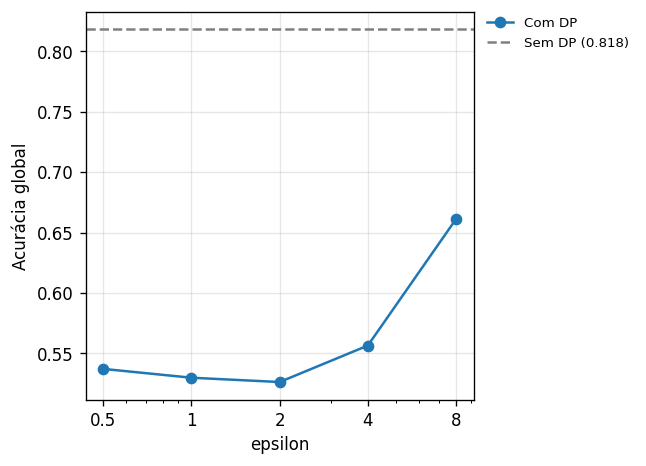
\includegraphics[width=0.46\linewidth]{figures/acuracia_vs_epsilon.png}}
\hfill
\subfigure[Recall e F1 da classe de falha]{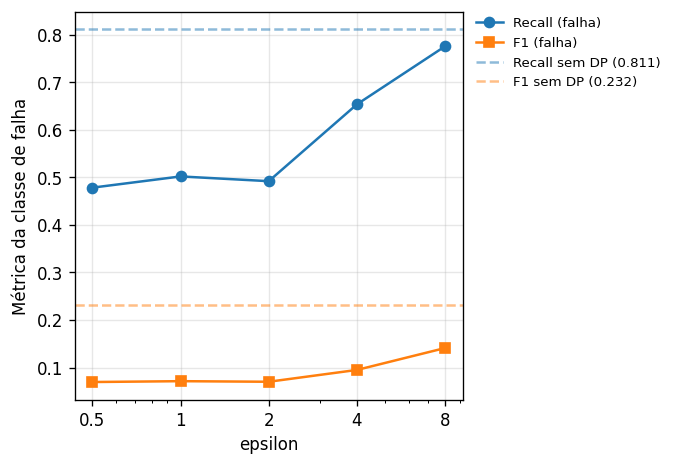
\includegraphics[width=0.46\linewidth]{figures/recall_f1_vs_epsilon.png}}
\caption{Utilidade do modelo em função de $\epsilon$ (escala logarítmica). A linha
tracejada marca o desempenho sem privacidade diferencial.}
\label{fig:util}
\end{figure}

\subsection{Convergência}

A Figura \ref{fig:conv} acompanha a perda e a acurácia ao longo das 20 rodadas. Sem
ruído, a perda cai e estabiliza próxima de $0{,}40$, e a acurácia sobe e se mantém
acima de $0{,}80$. Com privacidade diferencial, o ruído somado a cada rodada impede a
convergência suave: as curvas oscilam e param em níveis mais baixos. O caso
$\epsilon=8$, de menor ruído, mostra a menor oscilação entre as configurações
protegidas.

\begin{figure}[H]
\centering
\subfigure[Perda (log-loss)]{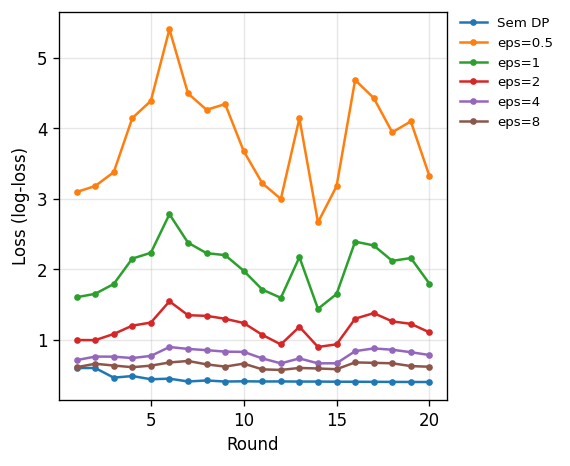
\includegraphics[width=0.46\linewidth]{figures/loss_vs_rounds.png}}
\hfill
\subfigure[Acurácia global]{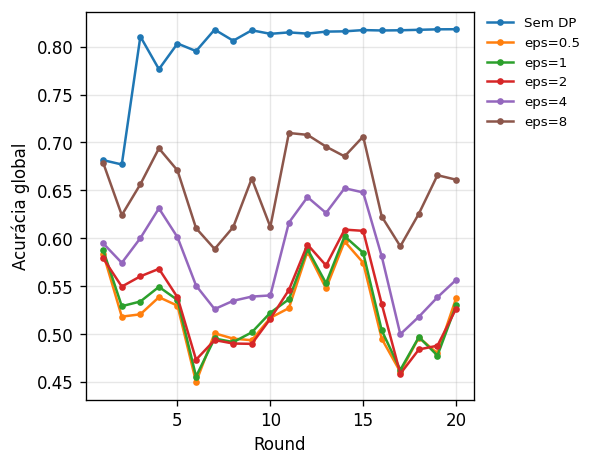
\includegraphics[width=0.46\linewidth]{figures/acuracia_vs_rounds.png}}
\caption{Evolução da perda e da acurácia por rodada, sem privacidade diferencial e
para três orçamentos $\epsilon$.}
\label{fig:conv}
\end{figure}

\subsection{Sensibilidade aos hiperparâmetros}

As Tabelas \ref{tab:clip}, \ref{tab:delta} e \ref{tab:rounds} isolam o efeito do limite
$C$, da folga $\delta$ e do número de rodadas, com $\epsilon=1$ fixo. O limite $C$
altera o ruído pela Equação \ref{eq:sigma} ($\sigma$ cresce com $C$), mas a
acurácia varia pouco (de $0{,}530$ a $0{,}531$), pois o recorte e o ruído se
compensam. A folga $\delta$ produz efeito pequeno: $\delta=10^{-7}$ aumenta $\sigma$
para $4{,}01$ e mantém a acurácia em $0{,}532$. O número de rodadas troca utilidade
por orçamento total: cinco rodadas gastam $\epsilon$ total de cinco e alcançam
$0{,}536$, enquanto 20 rodadas gastam 20 e alcançam $0{,}530$.

\begin{table}[H]
\centering
\caption{Efeito do limite de norma $C$ ($\epsilon=1$, $\delta=10^{-5}$, 20 rodadas).}
\label{tab:clip}
\small
\begin{tabular}{cccccc}
\toprule
$C$ & $\sigma$ & Acurácia & Recall (falha) & F1 (falha) & AUC do ataque \\
\midrule
0,5 & 1,70 & 0,531 & 0,482 & 0,069 & 0,505 \\
1   & 3,39 & 0,530 & 0,502 & 0,072 & 0,508 \\
2   & 6,79 & 0,530 & 0,483 & 0,069 & 0,511 \\
\bottomrule
\end{tabular}
\end{table}

\begin{table}[H]
\centering
\caption{Efeito da folga $\delta$ ($\epsilon=1$, $C=1$, 20 rodadas).}
\label{tab:delta}
\small
\begin{tabular}{cccccc}
\toprule
$\delta$ & $\sigma$ & Acurácia & Recall (falha) & F1 (falha) & AUC do ataque \\
\midrule
$10^{-3}$ & 2,63 & 0,530 & 0,461 & 0,067 & 0,507 \\
$10^{-5}$ & 3,39 & 0,530 & 0,502 & 0,072 & 0,508 \\
$10^{-7}$ & 4,01 & 0,532 & 0,508 & 0,073 & 0,509 \\
\bottomrule
\end{tabular}
\end{table}

\begin{table}[H]
\centering
\caption{Efeito do número de rodadas ($\epsilon=1$, $C=1$, $\delta=10^{-5}$).}
\label{tab:rounds}
\small
\begin{tabular}{ccccc}
\toprule
Rodadas & $\epsilon$ total & Acurácia & Recall (falha) & F1 (falha) \\
\midrule
5  & 5  & 0,536 & 0,454 & 0,056 \\
10 & 10 & 0,522 & 0,566 & 0,084 \\
20 & 20 & 0,530 & 0,502 & 0,072 \\
\bottomrule
\end{tabular}
\end{table}

\subsection{Eficácia do ataque}

A Tabela \ref{tab:atk} e a Figura \ref{fig:atk} medem a eficácia do ataque LiRA. Sem
privacidade diferencial, o ataque alcança AUC de $0{,}528$, pouco acima do acaso
($0{,}500$). A privacidade diferencial aproxima o ataque do acaso: em $\epsilon=1$, a
AUC cai para $0{,}508$, e o valor permanece entre $0{,}504$ e $0{,}511$ em todo o
intervalo de $\epsilon$, inclusive nos orçamentos altos que quase não somam ruído. A
Figura \ref{fig:atk}(b) compara o ataque sem proteção e com $\epsilon=1$ e confirma a
redução.

\begin{table}[H]
\centering
\caption{Eficácia do ataque LiRA conforme $\epsilon$ ($C=1$, $\delta=10^{-5}$). A AUC
e a acurácia balanceada valem $0{,}500$ no acaso.}
\label{tab:atk}
\small
\begin{tabular}{lccc}
\toprule
$\epsilon$ & $\sigma$ & AUC & Acurácia balanceada \\
\midrule
sem DP & --- & 0,528 & 0,554 \\
0,5 & 6,79 & 0,511 & 0,546 \\
1   & 3,39 & 0,508 & 0,545 \\
2   & 1,70 & 0,506 & 0,543 \\
4   & 0,85 & 0,505 & 0,544 \\
8   & 0,42 & 0,504 & 0,545 \\
16  & 0,21 & 0,505 & 0,542 \\
32  & 0,11 & 0,506 & 0,540 \\
64  & 0,05 & 0,506 & 0,540 \\
\bottomrule
\end{tabular}
\end{table}

\begin{figure}[H]
\centering
\subfigure[AUC do ataque por $\epsilon$]{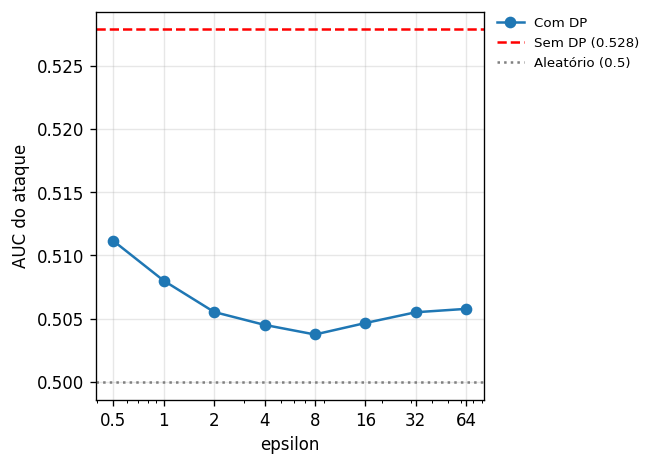
\includegraphics[width=0.46\linewidth]{figures/ataque_auc_vs_epsilon.png}}
\hfill
\subfigure[Ataque sem e com DP ($\epsilon=1$)]{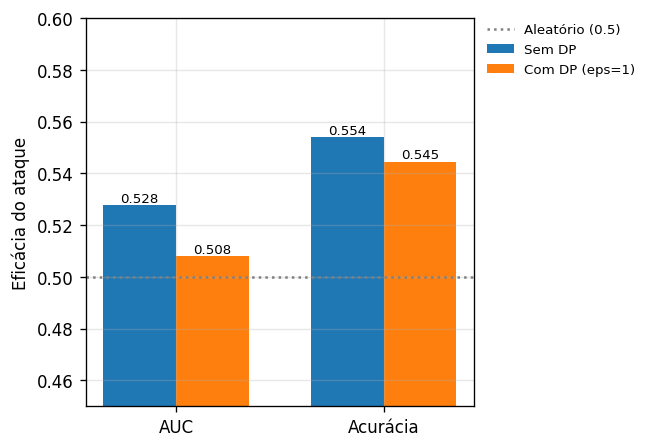
\includegraphics[width=0.46\linewidth]{figures/ataque_com_vs_sem_dp.png}}
\caption{Eficácia do ataque LiRA. A linha pontilhada marca o acaso ($0{,}500$) e a
tracejada, o ataque sem privacidade diferencial.}
\label{fig:atk}
\end{figure}

\subsection{Discussão}

O ataque revela pouca informação mesmo sem proteção, e dois fatores explicam esse
resultado. Primeiro, a regressão logística tem capacidade baixa e não memoriza
registros individuais. A inferência de pertencimento depende dessa memorização,
frequente em modelos superparametrizados e ausente aqui. Segundo, os atributos de
sensores descrevem regimes de operação compartilhados entre máquinas, o que reduz a
influência de um registro específico sobre os parâmetros. O modelo, portanto, já resiste
ao ataque por construção, e a privacidade diferencial acrescenta uma garantia formal
sobre essa resistência.

A métrica empírica do ataque não ordena, por si, o nível de privacidade: a AUC
permanece próxima de $0{,}50$ para qualquer $\epsilon$, o que impede concluir que
um orçamento supere outro a partir desse número. A ordenação vem da garantia formal:
um $\epsilon$ menor aproxima as distribuições da Equação \ref{eq:dp} e protege mais,
independentemente da força do ataque. A privacidade diferencial oferece, assim, uma
proteção de pior caso que o ataque empírico não consegue medir neste cenário.

\section{Conclusão} \label{sec:conc}

Este trabalho construiu um sistema de aprendizado federado com privacidade
diferencial para a previsão de falhas industriais e mediu o compromisso entre
privacidade e utilidade. O mecanismo gaussiano, com recorte da norma L2 e ruído
calibrado por $\epsilon$, protege a participação de cada fábrica a cada rodada sem
mover os dados. A avaliação quantificou a queda de utilidade conforme o orçamento
diminui (de $0{,}818$ de acurácia sem proteção a $0{,}537$ em $\epsilon=0{,}5$)
e confirmou, com o ataque LiRA, que a proteção empurra a inferência de pertencimento
para o nível do acaso.

O cenário também revela limites. A regressão logística resiste ao ataque por
construção, o que reduz a margem observável da privacidade diferencial. Modelos de
maior capacidade mostrariam um ganho mais claro. A contagem de orçamento adota a
composição sequencial, conservadora frente a métodos como a privacidade diferencial
de Rényi \cite{mironov2017renyi}. A avaliação de utilidade mede as métricas sobre os dados
locais de treino, sem um conjunto de teste separado. O conjunto AI4I 2020, por fim, reproduz
dados sintéticos. Trabalhos futuros
apontam três direções: classificadores mais expressivos, contabilidade de orçamento
mais precisa e agregação segura no servidor, que somaria sigilo da comunicação à
proteção dos parâmetros.

\bibliographystyle{sbc}
\bibliography{references}

\end{document}
